% pgfplots line plot with two series + legend.
% Requires: \usepackage{pgfplots} and \pgfplotsset{compat=newest}

\begin{frame}{Training curves}
    \begin{tikzpicture}
        \begin{axis}[
            width=0.75\textwidth, height=0.6\textheight,
            xlabel={Epoch}, ylabel={Validation loss},
            grid=major,
            legend pos=north east,
            legend cell align=left,
        ]
            % Series 1: inline data
            \addplot[blue, thick, mark=*] coordinates {
                (0, 1.20) (10, 0.85) (20, 0.62) (30, 0.48)
                (40, 0.39) (50, 0.34) (60, 0.32) (70, 0.31)
            };
            \addlegendentry{Method A}

            % Series 2: linear fit overlay
            \addplot[red, dashed, thick] coordinates {
                (0, 1.20) (10, 0.95) (20, 0.78) (30, 0.66)
                (40, 0.58) (50, 0.52) (60, 0.48) (70, 0.45)
            };
            \addlegendentry{Baseline}

            % Optional: external data file
            % \addplot[green!60!black, thick] table[x=epoch, y=loss] {data.dat};
            % \addlegendentry{Method C}
        \end{axis}
    \end{tikzpicture}
\end{frame}
